\section{Schlussfolgerungen}
\label{sec:schlussfolgerungen}

Siehe Tabelle~\ref{tab:uebersicht} auf Seite~\pageref{tab:uebersicht}.

\begin{wichtigbox}
Kurze Zusammenfassung der \enquote{Ergebnisse}, bzw. Auflisten der Vorteile
wenn man sich an die genannten Best Practices hällt. Dabei kann man sich auch
stark an dem Abstract orientieren.
\end{wichtigbox}

\begin{table}[htbp]
    \centering
        \caption{Übersicht über die Best Practices}
        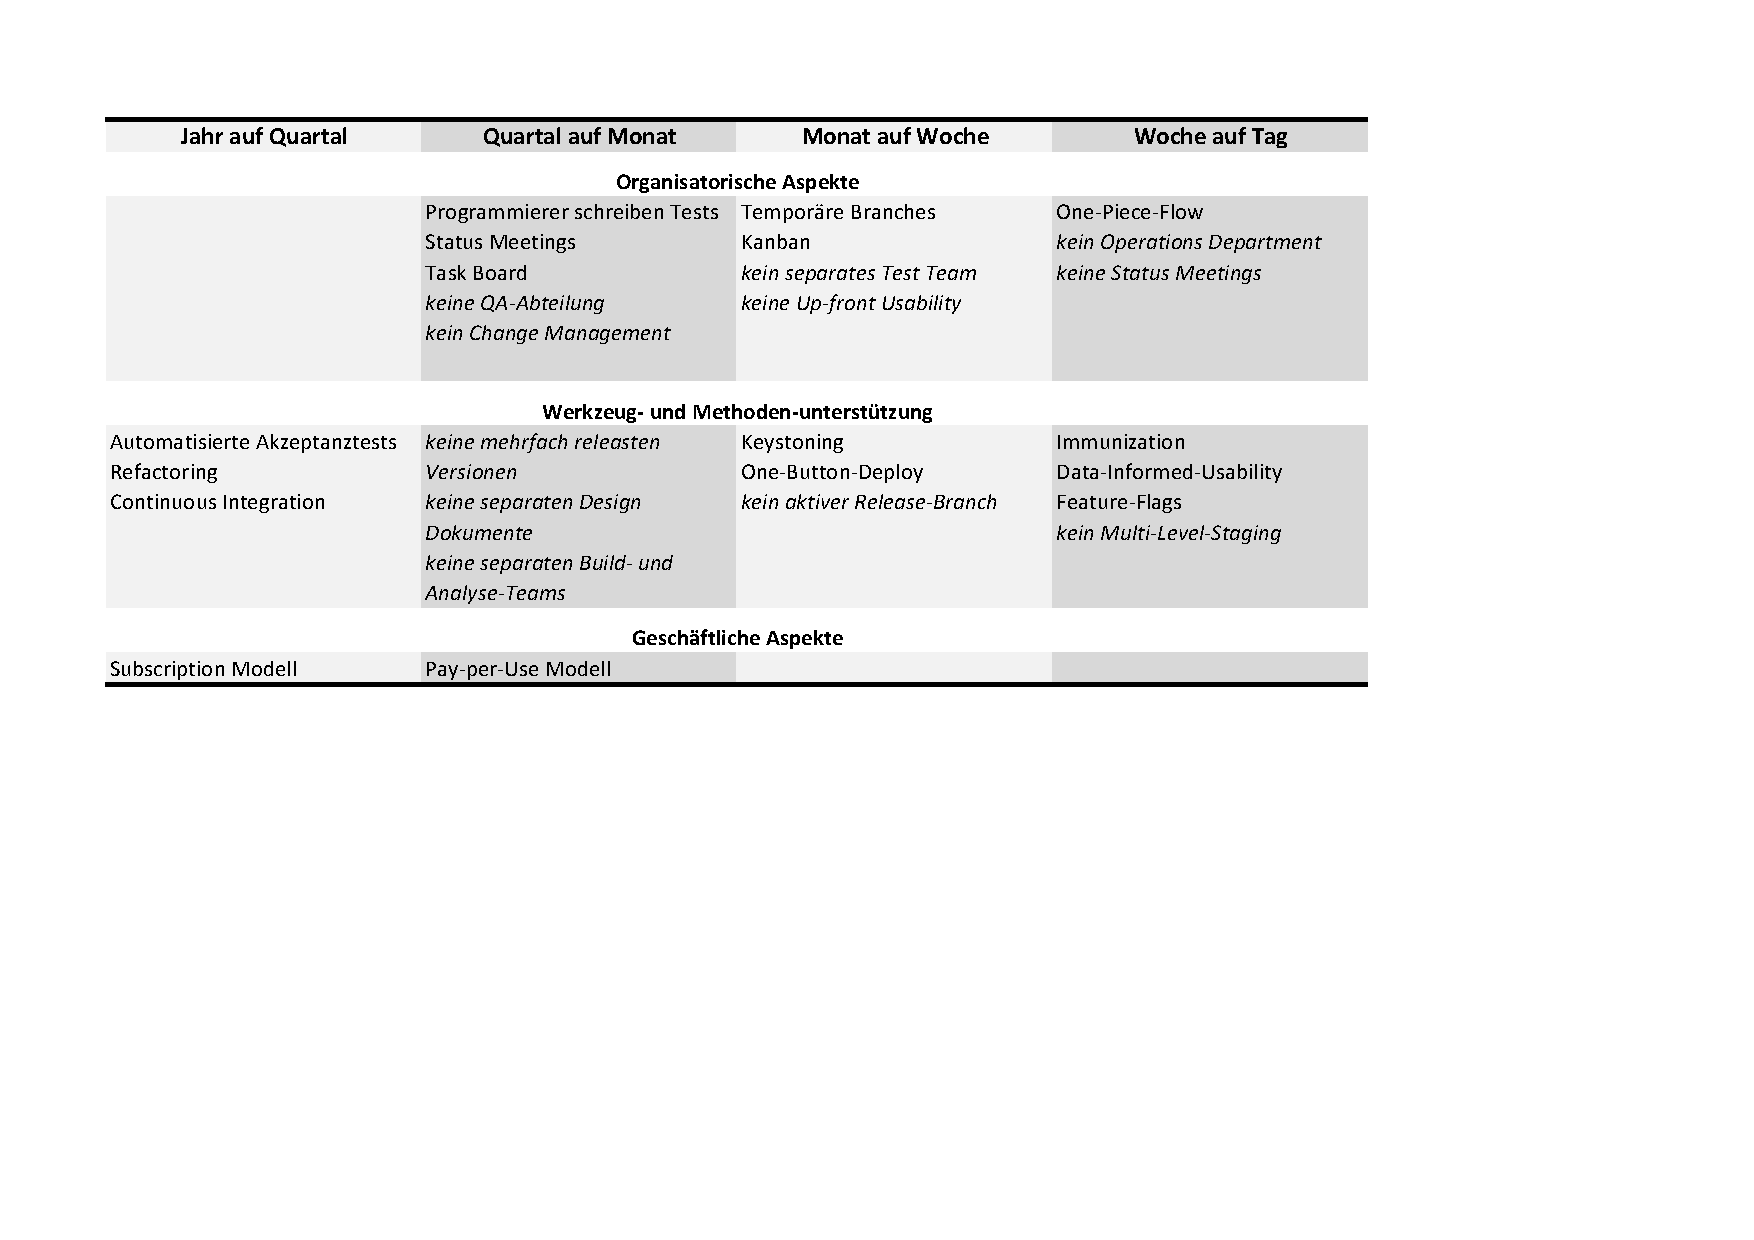
\includegraphics[trim = 50bp 265bp 185bp 56bp, clip, width=1.00\textwidth]{uebersicht}
    \label{tab:uebersicht}
\end{table}


\begin{quote}
\zitat{Does this mean we're never going to introduce bugs to our live site? Of
course not - but we're going to keep the number of bugs to hit the live site
to a minimum, and we've made it easy and fast to get bug fixes live as
well.}~\cite{digg4}
\end{quote}
